
%!TEX root = ../dissertation.tex

\chapter{Conclusions}
\label{chap:conclusions}
In this thesis, the numerical modeling and simulation of multi-physics mechanical systems consisting of discrete and continua were investigated via Lagrangian methods.  Specifically, 
\begin{enumerate}[(a)]
	\item Rigid and flexible multi-body dynamic systems featuring frictional contact were studied.  The former was employed in granular material simulations while the later was used in the simulation of articular cartilage during the gait cycle.
	\item The dynamics of continua were investigated for fluid dynamics problems and for continuum simulation of granular flows. The continuum modeling of granular flows allowed for modeling such materials via a computationally less expensive method than the DEM counterpart.
	\item The coupling between continuum and discrete sub-systems was investigated primarily for fluid-solid interaction problems. 	
\end{enumerate}
 The HPC approach employed in this thesis draws on hybrid multi-core shared memory architecture for discrete systems and GPU computing for the continua. The software implementation of the framework is part of an open-source software and is available on public domains.

Verification and validation of the different aspects of the numerical method were conducted through comparison with experimental results or other well-established numerical methods. The  multi-physics framework was used in studying real-world problems, including $(i)$ the relation between loading and the articular cartilage split-line patterns, $(ii)$ fluid-solid interaction in compliant and under-water robotic applications, and $(iii)$ continuum modeling of granular material.  

The developments made as part of this thesis work provide a robust foundation for coupling rigid bodies, fluids and flexible objects in a fully Lagrangian framework. Traditional Eulerian approaches for such multi-physics coupling involve tracking implicit surfaces through the continuum or re-meshing the domain frequently throughout the simulation. The Lagrangian alternative proposed in this work is more robust for multi-physics problems that involve large displacement and deformation in the discrete system.

The specific contributions of the author are summarized as follows:
\begin{compactitem} 
	\item Investigated the use of SPH for the Navier-Stokes equations
	\begin{compactitem} 
		\item Investigated four different SPH methods (WCSPH, ISPH, KCSPH, and IISPH) and  their solution attributes
		\item Performed a comparison between Implicit SPH (ISPH), Weakly Compressible SPH (WCSPH), and Kinematically Constrained SPH (KCSPH)
		\item Compared and contrasted the solution attributes of SPH as a Lagrangian method against continuous finite element method for free-surface and fluid-solid interaction problems 
		\item Implemented and improved the Implicit Incompressible SPH \cite{ihmsen2014implicit} method by solving the discretized Poisson pressure equation via advanced linear solvers
		\item Implemented and validated a projection-based implicit, both velocity and pressure, solver that can handle a wide range of fluid flows ranging from highly viscous flows to flows with moderately large Reynolds numbers in the laminar regime
		\item Investigated the use of consistent SPH discretization for internal flow problems
		\item Implemented the Herschel-Bulkley fluid model for modeling and simulation of non-Newtonian fluids
		\item Investigated the use of ISPH method for modeling and simulation of granular dynamics as a non-Newtonian fluid 
	\end{compactitem}
	
	
	\item Investigated the solution quality in frictional-contact problems and demonstrated insights gained in the context of a biomechanics application 
	\begin{compactitem} 
		\item  Investigated the use of the Tikhonov regularization method for imparting uniqueness to the distribution of frictional contact forces in granular dynamics problems solved via a differential variational inequality approach
		\item Simulated the tibiofemoral cartilage contact during walking for the prediction of collagen fiber orientation
	\end{compactitem}
	
	\item Developed a partitioned fluid-solid interaction framework
	\begin{compactitem} 
		\item  Coupled the fluid solver to a multi-body engine capable of simulating rigid and flexible bodies  interacting through frictional contact
		\item  Validated the fluid-structure coupling via benchmark experiments featuring flexible and rigid elements
	\end{compactitem}
	
	
	\item Leveraged hybrid CPU/GPU parallelization to improve the performance of the FSI framework 
	\begin{compactitem} 
		\item Implemented SPH on GPU cards using CUDA  to leverage high memory bandwidth
		\item Implemented Krylov linear solvers such as GMRES and BiCGStab on GPU to improve the efficiency of the underlying linear solvers
		\item Leveraged OpenMP for parallelism of the flexible multi-body dynamics solver on the CPU
		\item Improved the efficiency of the low-level matrix operation on the host code via AVX vectorization intrinsics
	\end{compactitem}
\end{compactitem} 

\section{Statement of Acknowledgment}
 This work was supported by National Institutes of Health [grant number EB015410] and National Science Foundation [grant number CMMI 1635004]. The development of the  multi-physics platform discussed in this thesis employed the work of previous authors as follows:
\begin{itemize}
	\item The WCSPH formulation discussed in \S\ref{sec:WCSPH} adopt the  implementation of the previous work discussed in \cite{PazoukiPhDThesis2014}.
	\item The KCSPH formulation discussed in \S\ref{sec:KCSPH} employed the implementation of the previous work  discussed in \cite{hammadPhDThesis}.
	\item The multi-body and the rigid body formulation discussed in \S\ref{sec:RigidBody} and \S\ref{sec:FMBD} employed Chrono \cite{chronoOverview2016,chronoOverview2013}.
	\item The development of the articular cartilage model discussed in \S\ref{sec:AC_model} was conducted in collaboration with the co-authors of the paper published in \cite{rakhsha2019simulation}.  Tibio-femoral kinematics during walking explained in \S\ref{ss:ComputationalAC} employed the data published in \cite{Smith2016,Smith2016influence2}.
\end{itemize} 

\section{Future Direction of Research}
The future directions of research involve solving more challenging real-world problems with the current framework as well as improving the numerical methods employed in this work. Details are provided in the next three subsections.
%\section{Data Driven CFD}
\subsection{Hybrid Eulerian-Lagrangian Discretization: MPM}
Material Point Method (MPM) is a hybrid Eulerian-Lagrangian discretization that can be used to space-discretize a wide range of problems from fluids to solids.  MPM was first described in \cite{sulsky1994particle}, and is a derivative of the fluid-implicit-particle (FLIP) method \cite{brackbill1988flip}, which is based on the particle-in-cell (PIC) method \cite{harlow1964particle}. The key idea of MPM is to store the state variables on Lagrangian material points, while the equations of motion are solved on a background grid.  More specifically, in MPM the body is discretized with a set of \textit{material points} placed on a \textit{background grid}, which is used for computation of the gradient terms. Some of the problems associated with mesh-based methods for FSI applications (see \S\ref{sec:FSI_intro})  are not encountered in MPM; this is because the re-meshing step is not necessary, making  MPM suitable for modeling problem involving large deformations. At the beginning of the MPM  simulation, the grid is initialized such that it includes the continuum body. The material points are distributed on the continuum body as well. During each time-step, the MPM algorithm can be summarized in the following steps:
\begin{enumerate}
	\item  Quantities such as mass, velocity, internal and external forces are extrapolated from the material points to the grid nodes using the shape functions as: 
	\begin{equation}
	\phi^i_{node}=\sum_{p \in \support{node\;i}} \phi^p_{mp} N_{mp-nd}(\vect{x}_{ip}),
	\end{equation}
	where $N_{mp-nd}(\vect{x}_{ip})$ is the interpolation function from the \textit{material points} to the grid \textit{nodes}.
	\item Equations of motion with proper constitutive relations are solved on the grid for velocity and acceleration. The mesh nodes are advected and required gradients are calculated on the grid. 
	\item Grid node quantities are extrapolated back to the material points according to 
	\begin{equation}
	\phi^p_{mp}=\sum_{i \in \support{node\;p}} \phi^i_{mp} N_{nd-mp}(\vect{x}_{pi}),
	\end{equation}
	where $N_{nd-mp}(\vect{x}_{pi})$ is the interpolation function from the grid \textit{nodes} to the \textit{material points}.
	\item The distorted grid is reseted to a uniform grid encompassing the continuum body for the next time step.
\end{enumerate} 


\subsection{Higher-order Lagrangian Discretization: GMLS}
SPH is a robust mesh-less method for a wide range of problems, especially for fluid-solid interaction problems involving large displacement and deformation. However, instability/accuracy concerns are associated with each of the SPH methods discussed in sections \S\ref{sec:Space-Discretization} at high/low Reynolds numbers. 
The idea behind the Generalized Moving Least Squares method is to reconstruct a function from an unstructured set of point data sampled in a neighborhood of any point in space. Specifically, if the function $\psi(\vect{x})$ is to be approximated by a $m^{th}$-order polynomial from its point data values $\psi_j$ in some neighborhood of $\vect{x}$, the GMLS approximation of $\psi(\vect{x})$ is as follows:
\begin{equation}
\psi(\vect{x_i})=\vect{P}^T_i(\vect{x}_i) \vect{c}^*_i,
\end{equation}
where $\vect{c}^*_i$ is the unknown polynomial coefficient vector that is obtained through minimization of a weighted residual functional, e.g., $\sum_{j \in \support{i}} \big(\psi_j - \vect{P}^T_i(\vect{x}_j) \vect{c}_i\big)^2W_{ij}$. Above, $\vect{P}$ is the polynomial basis vector, e.g., $\vect{P}=[1,x,y,x^2,xy,y^2]$ in 2D for $m=2$, which introduces 6 unknowns in the coefficient vector $\vect{c}^*_i$. After taking the variation with respect to $\vect{c}_i$, it follows that:
\begin{equation}
\vect{c}^{*}_{i}= \vect{M}_i^{-1}\Big( \sum_{j \in \support{i}} \vect{P}_i(\vect{x}_j) W_{ij}  \psi_j \Big), 
\end{equation}
where 
\begin{equation}
\vect{M}_i=  \sum_{j \in \support{i}}  \vect{P}_i(\vect{x}_j) W_{ij}  \vect{P}^T_i(\vect{x}_j).
\end{equation}
The GMLS procedure introduces a way for optimal recovery of linear target functionals over a desired reproduction space. See \cite{hu2019spatially, trask2016compact} for more details about this method.
 
\subsection{Biomechanics Applications: Articular Cartilage}
Osteoarthritis (OA), the breakdown of the articular cartilage, affects the lives of millions of adults. Although there are treatments to manage the condition, there is no cure nor any completely effective method of preventing the disease. As such, it is essential to comprehensively study factors that contribute to OA in order to guide the development of improved treatments. Research in this field has the potential to substantially improve our understanding of multi-scale articular cartilage mechanics, which assists efforts to investigate degenerative pathways. The focus of this direction of future research is  on the modeling and simulation of the micro-structure of the articular cartilage. 

Structurally, cartilage consists of two distinct phases: a fluid phase, composed of water and electrolytes, and a solid phase, composed of collagen fibrils, chondrocytes, and proteoglycans \cite{Mow1992}. The micro-structure of the cartilage is shown in figure \ref{fig:AC}.
Figure~\ref{fig:AC} demonstrates the proposed FSI modeling strategy. 
\begin{figure}[H]
	\centering
	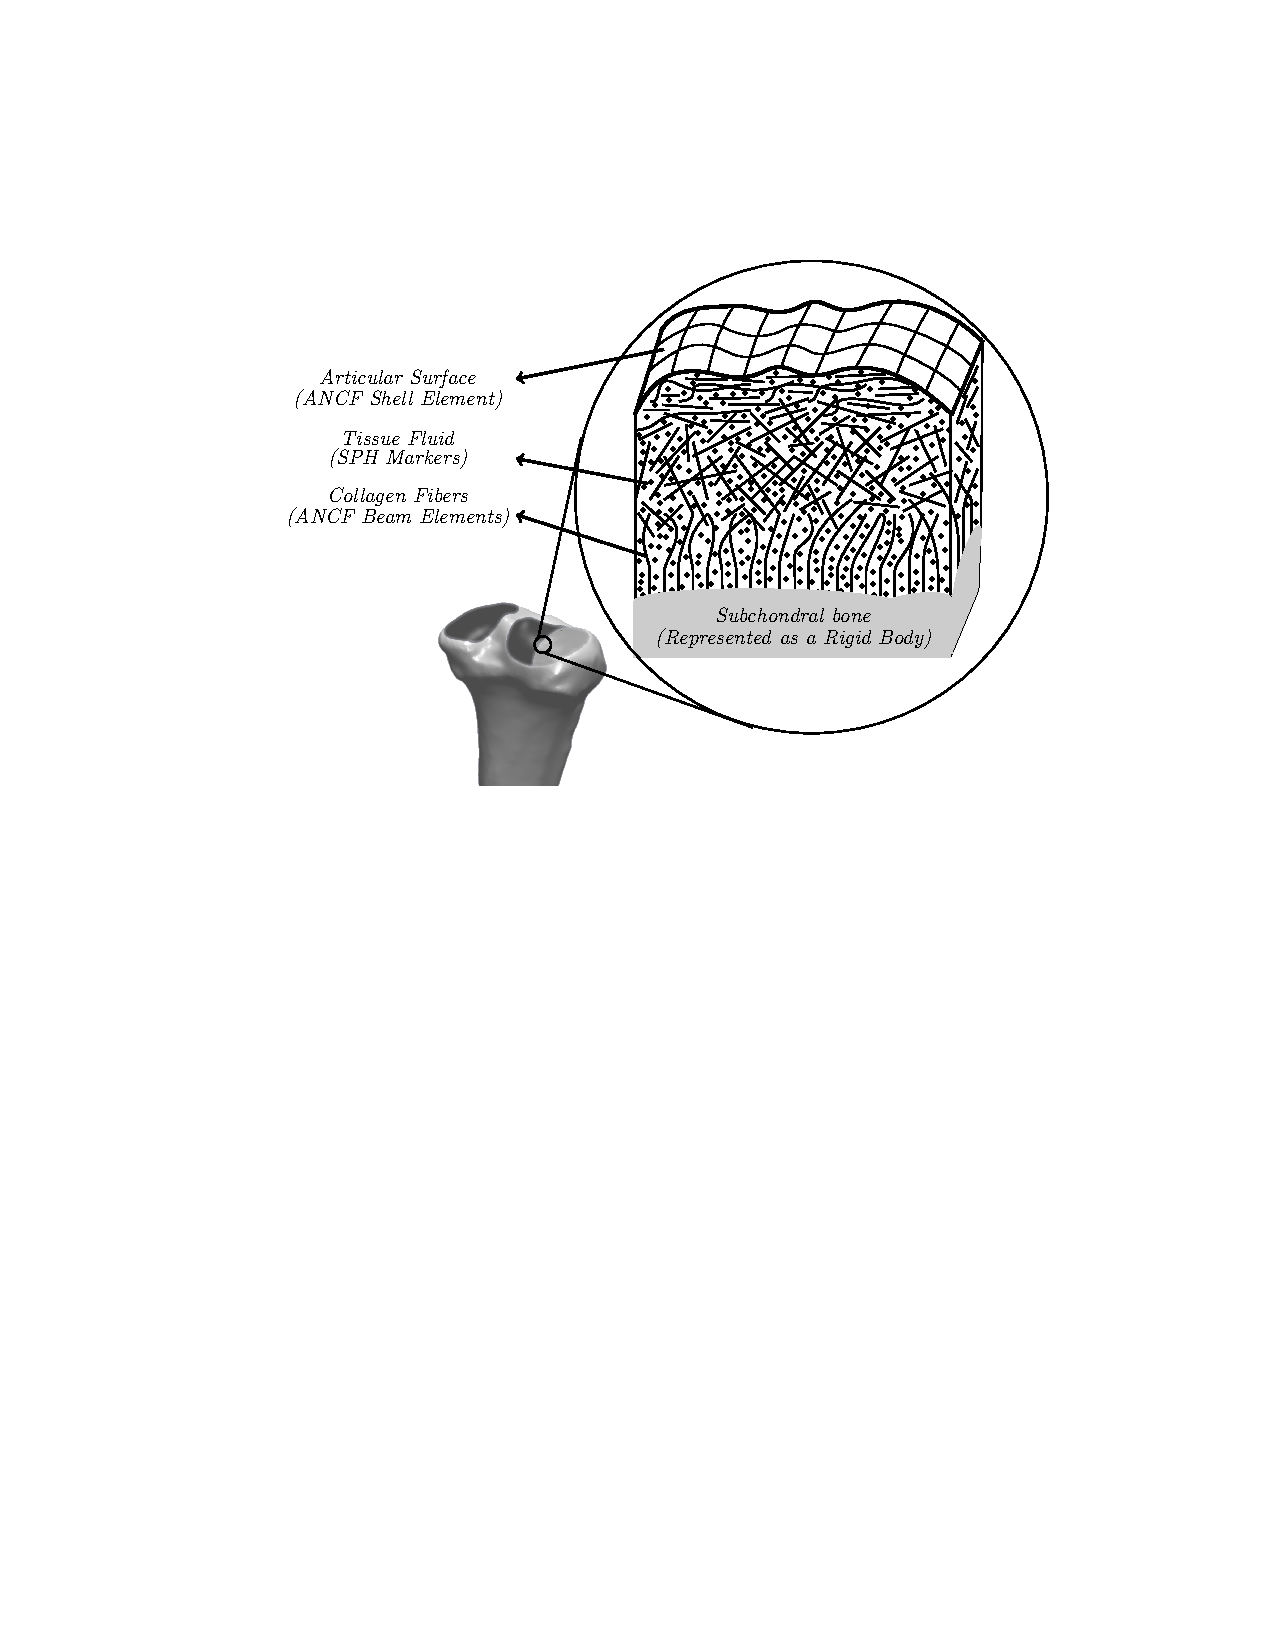
\includegraphics[width=0.7\linewidth]{images/AC.pdf}
	\captionof{figure}{Fluid-solid interaction modeling strategy of the articular cartilage}
	\label{fig:AC}
\end{figure}
The substantial load-bearing capacity of this multiphase tissue is provided by complex interactions between its solid network of collagen fibers and macromolecules, and the interstitial fluid. In an unloaded state, an electrostatic attraction between the proteoglycan macromolecules and the interstitial fluid leads to an osmotic pressurization of the tissue. This internal pressure is equilibrated by tensile loading in the collagen fibers. When cartilage is compressed, the contact loads are distributed throughout the tissue via further pressurization of the interstitial fluid \cite{Cohen1998, Fox2009}.


The behavior of articular cartilage (AC) can be analyzed on several scales. On the macroscopic level, the cartilage is a small layer, few millimeters thick, that lubricates the relative motion among body parts. On the micro-scale level ($10^{-7}$\,m--$10^{-4}$\,m), the density and orientation of collagen fibrils vary with the depth within the cartilage. One level down, on the ultra-scale ($10^{-8}$\,m--$10^{-6}$\,m), proteoglycans and individual collagen fibrils of up to 200\,nm in diameter interact electrostatically and mechanically.\\ The mechanics of AC has been modeled in the literature through continuum-based representations using either biphasic or triphasic formulations, relying on constitutive properties derived from experimental observations~\cite{Li2009,halloran2012multiscale}. These formulations use the methods of composite materials for giving directional properties to the cartilage. While these approaches provide a holistic view of the tissue, they do not explicitly model the discrete fluid-solid interactions (FSI) on the ultra-scale level. The future investigation involves an FSI approach to model the microstructure of the articular cartilage using the fundamental elements described above. Modeling articular cartilage on the ultra-scale level through a discrete, fully coupled representation of fluid and solids provides more accurate insight into the biomechanical properties of the AC. This direction of future research allows for deepening our understanding of how macroscopic behavior is affected by the interplay of microstructural elements. 
Preliminary results of the small-scale FSI model for a confined compression test are demonstrated in Figure~\ref{fig:IR}.
\begin{figure}[H]
	\centering
		\centering	
	\begin{subfigure}{1.0\columnwidth}	
		\centering
		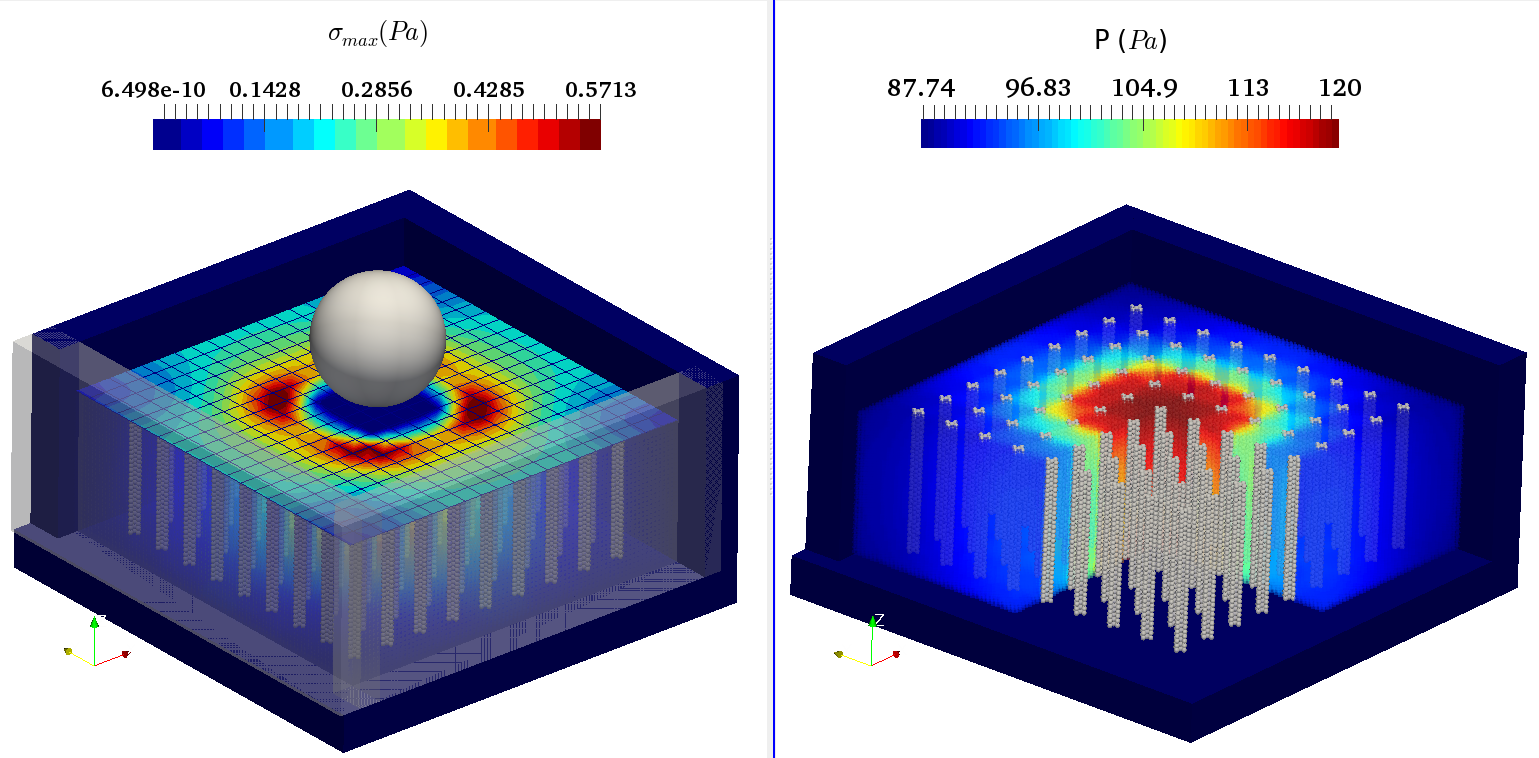
\includegraphics[width=0.8\linewidth]{images/fibers.png}
	\end{subfigure}	

	\begin{subfigure}{1.0\columnwidth}	
		\centering
		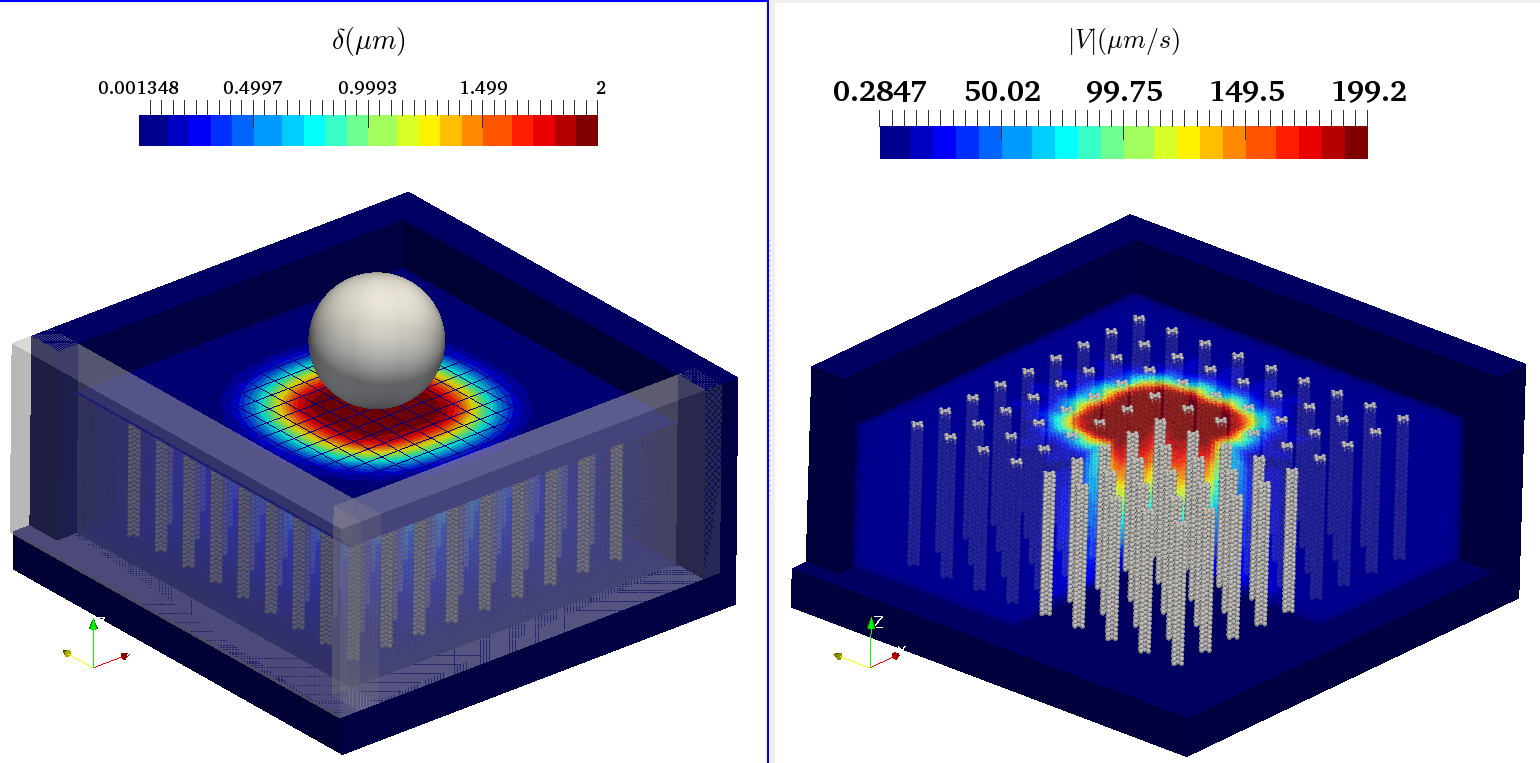
\includegraphics[width=0.8\linewidth]{images/fibers2.png}
	\end{subfigure}	
	\captionof{figure}{Preliminary results of the articular cartilage FSI model. Displacement and stress field on the articular surface (top and bottom left, respectively). Pressure and velocity distribution inside the interstitial fluid (top and bottom right, respectively)}
	\label{fig:IR}
\end{figure}